\section{Exciton-Polariton Topological Insulator with an Array of Magnetic Dots}\label{Ch5}

%\section{Background}
Robust transport of particles in topologically nontrivial systems follows from the existence of protected edge states at the interfaces between media having different topological properties~\cite{Hasan:2010aa,Qi:2011hb,Chiu:2016aa}.
Such edge modes are robust against disorder, which makes them appealing to both theoretical and experimental research. Phase transitions to topological insulating phases were originally discovered in the context of the integer quantum Hall effect~\cite{Klitzing:1980aa}, where a nonzero quantized Chern number is associated with disorder-robust quantization of the particle current in strong external magnetic fields.
Later this idea was extended to the anomalous quantum Hall and quantum spin Hall effects~\cite{Haldane:1988aa, Kane:2005aa, Bernevig:2006aa, Konig:2007aa}, where an external net magnetic field is not required. In these cases, the field is replaced by other effects such as time-reversal symmetry breaking from an internal magnetization of the material~\cite{Karplus:1954aa, Chang:2013aa} or strong spin-orbit coupling. Topological phases have now been extended to various physical systems, including photonics, cold atoms, and acoustics~\cite{Wang2009,Jotzu:2014aa, Yang:2015aa}.

Recently, an exciton-polariton topological Chern insulator has been demonstrated ~\cite{Klembt:2018aa}. In contrast to other systems, the nontrivial topological phase in this work arose from the following main features: an artificial lattice made of micrometer-sized pillars, excitonic spin-orbit coupling or photonic TE-TM splitting, and an external magnetic field in the Faraday configuration~\cite{Bardyn:2015aa, Nalitov:2015aa}. The effects are as follows. The lattice creates a finite Brillouin zone with energy bands in reciprocal space, the spin-orbit coupling creates a momentum-dependent energy splitting between spin states without opening a bandgap, and the external magnetic field induces a Zeeman splitting between spin-up and spin-down exciton-polaritons. All three effects are required to create a topological bandgap that contains the protected edge states, in contrast to other platforms, where a lattice combined with a uniform or staggered magnetic field is sufficient.

%One of the fascinating topics of research recently is nontrivial topology in artificial materials, which is caused by an external influence on a complex system, possessing certain internal properties.
% example, a celebrated exciton-polariton topological insulator~\cite{Klembt:2018aa, Karzig:2015aa, Bardyn:2015aa, Nalitov:2015aa} requires three main ingredients: first, an excitonic spin-orbital coupling or the photonic TE-TM splitting; second, localization due to the presence of an artificial lattice made of micrometer-sized pillars; and, third, an external magnetic field in the Faraday configuration.
%The lattice allows for the formation of the finite Brillouin zone and bands in the reciprocal space, the spin-orbital effects give the energy splitting between the spin-up and spin-down projections, and the magnetic field allows for the gap opening, where the edge state resides.

To date, theoretical and experimental works regarding exciton-polariton topological insulators have considered a uniform external magnetic field~\cite{Gulevich:2016aa,Nalitov:2015aa,Bardyn:2015aa,Yi:2016aa,PhysRevB.93.085438}.
In order to observe a measurable bandgap, a large external magnetic field has been employed, requiring superconducting coils and cryogenic temperatures~\cite{Klembt:2018aa}.
%
Such a strong external magnetic field is a significant drawback that limits potential applications in real devices.
In particular, the essential advantages of microcavity samples (e.g. their compactness and potential for room-temperature operation) are neutralized.
It is therefore crucial to explore application-friendly mechanisms and techniques by which topological polaritons can be created without an external magnetic field.


Existing proposals have been based on such effects as the nonlinear dynamics under resonant pumping~\cite{Mandal:2019aa}, time or spin-dependent pumping~\cite{Sigurdsson:2019aa}, and spontaneous symmetry breaking~\cite{Karzig:2015aa,Janot:2016aa}.
All these proposals, though, have technological limitations; for example, using the nonlinear terms due to particle interaction requires strong resonant pumping of the sample in order to excite the edge as a perturbation~\cite{Bardyn:2015aa,PhysRevB.93.085438}.
This spin-dependent pumping demands each lattice site to be treated independently, and this makes experimental design tricky.

The following sections introduce an easily realizable alternate design for an polariton topological insulator in which the external uniform magnetic field is replaced by an internal inhomogeneous magnetization, produced by a magnetic material (MM) embedded within the microcavity.
Such magnetic quantum dots are not only interesting by itself~\cite{Vavassori:2000aa}, the applications can found in superconductors~\cite{Erdin:2002aa,Otani:1993aa,Lyuskyutov:2005aa} and electron system~\cite{Li:2007aa}.
We show that the resulting staggered magnetic field is capable of opening a topological bandgap, and can yield topological transitions between different Chern numbers ($\pm 2$ to $\mp 1$) as either the magnetic field or spin-orbit coupling strength are varied, similar to the uniform external field case~\cite{Bleu:2017aa}.
Our approach can eliminate the need for superconducting coils and other equipment, thereby bringing practical device applications with exciton-polariton topological insulators closer.

%we propose a new design of an exciton-polariton topological insulator. We show that instead of using an external homogeneous magnetic field, a local magnetic moment can be created in the system to open the gap and give the topological phase transition from a topologically trivial case to a nontrivial one.
%Moreover, we show that there might occur a phase transition between two different topologically nontrivial configurations, and it corresponds to change of the Chern number from $\pm 2$ to $\mp 1$.


%----------------------
%----------------------
%----------------------

\subsection{System schematic}
Let us consider polaritons loaded in the honeycomb lattice shown in Fig.~\ref{fig:Ch5_Fig1}(a).
In recent experiments~\cite{Klembt:2018aa}, an external homogeneous magnetic field perpendicular to the lattice was applied to break time reversal symmetry.
To get rid of the setup required to generate a sufficiently strong magnetic field, we use an MM layer to represent an array of sub-micron magnetic QDs. When magnetized, they can replace an external field.
%Such MM arrays can be applied to ultrahigh-density magnetic recording media and devices to control superconductors~\cite{Baert:1995aa}.
%In this work, we apply this magnetic material (MM) in the exciton-polariton system to break the time reversal symmetry.
% Let us consider a polariton honeycomb lattice presented in Fig.~1(a), where instead of an external homogeneous magnetic field perpendicular to the 2D system, we put a layer of a magnetic material (MM) inside the cavity.
%
The first case to consider locates the MM on the pillars from the top, thus covering the upper DBR.
Then the MM represents an array of magnetic QDs [\ref{fig:Ch5_Fig1}(b)].
%{\bf DL: why not use a uniform coating of the MM? Is it because the MM also induces the honeycomb lattice structure?}{\color{blue} MM does not induce the honeycomb lattice structure.}
%
%
%
\begin{figure}[ht]
    \centering
	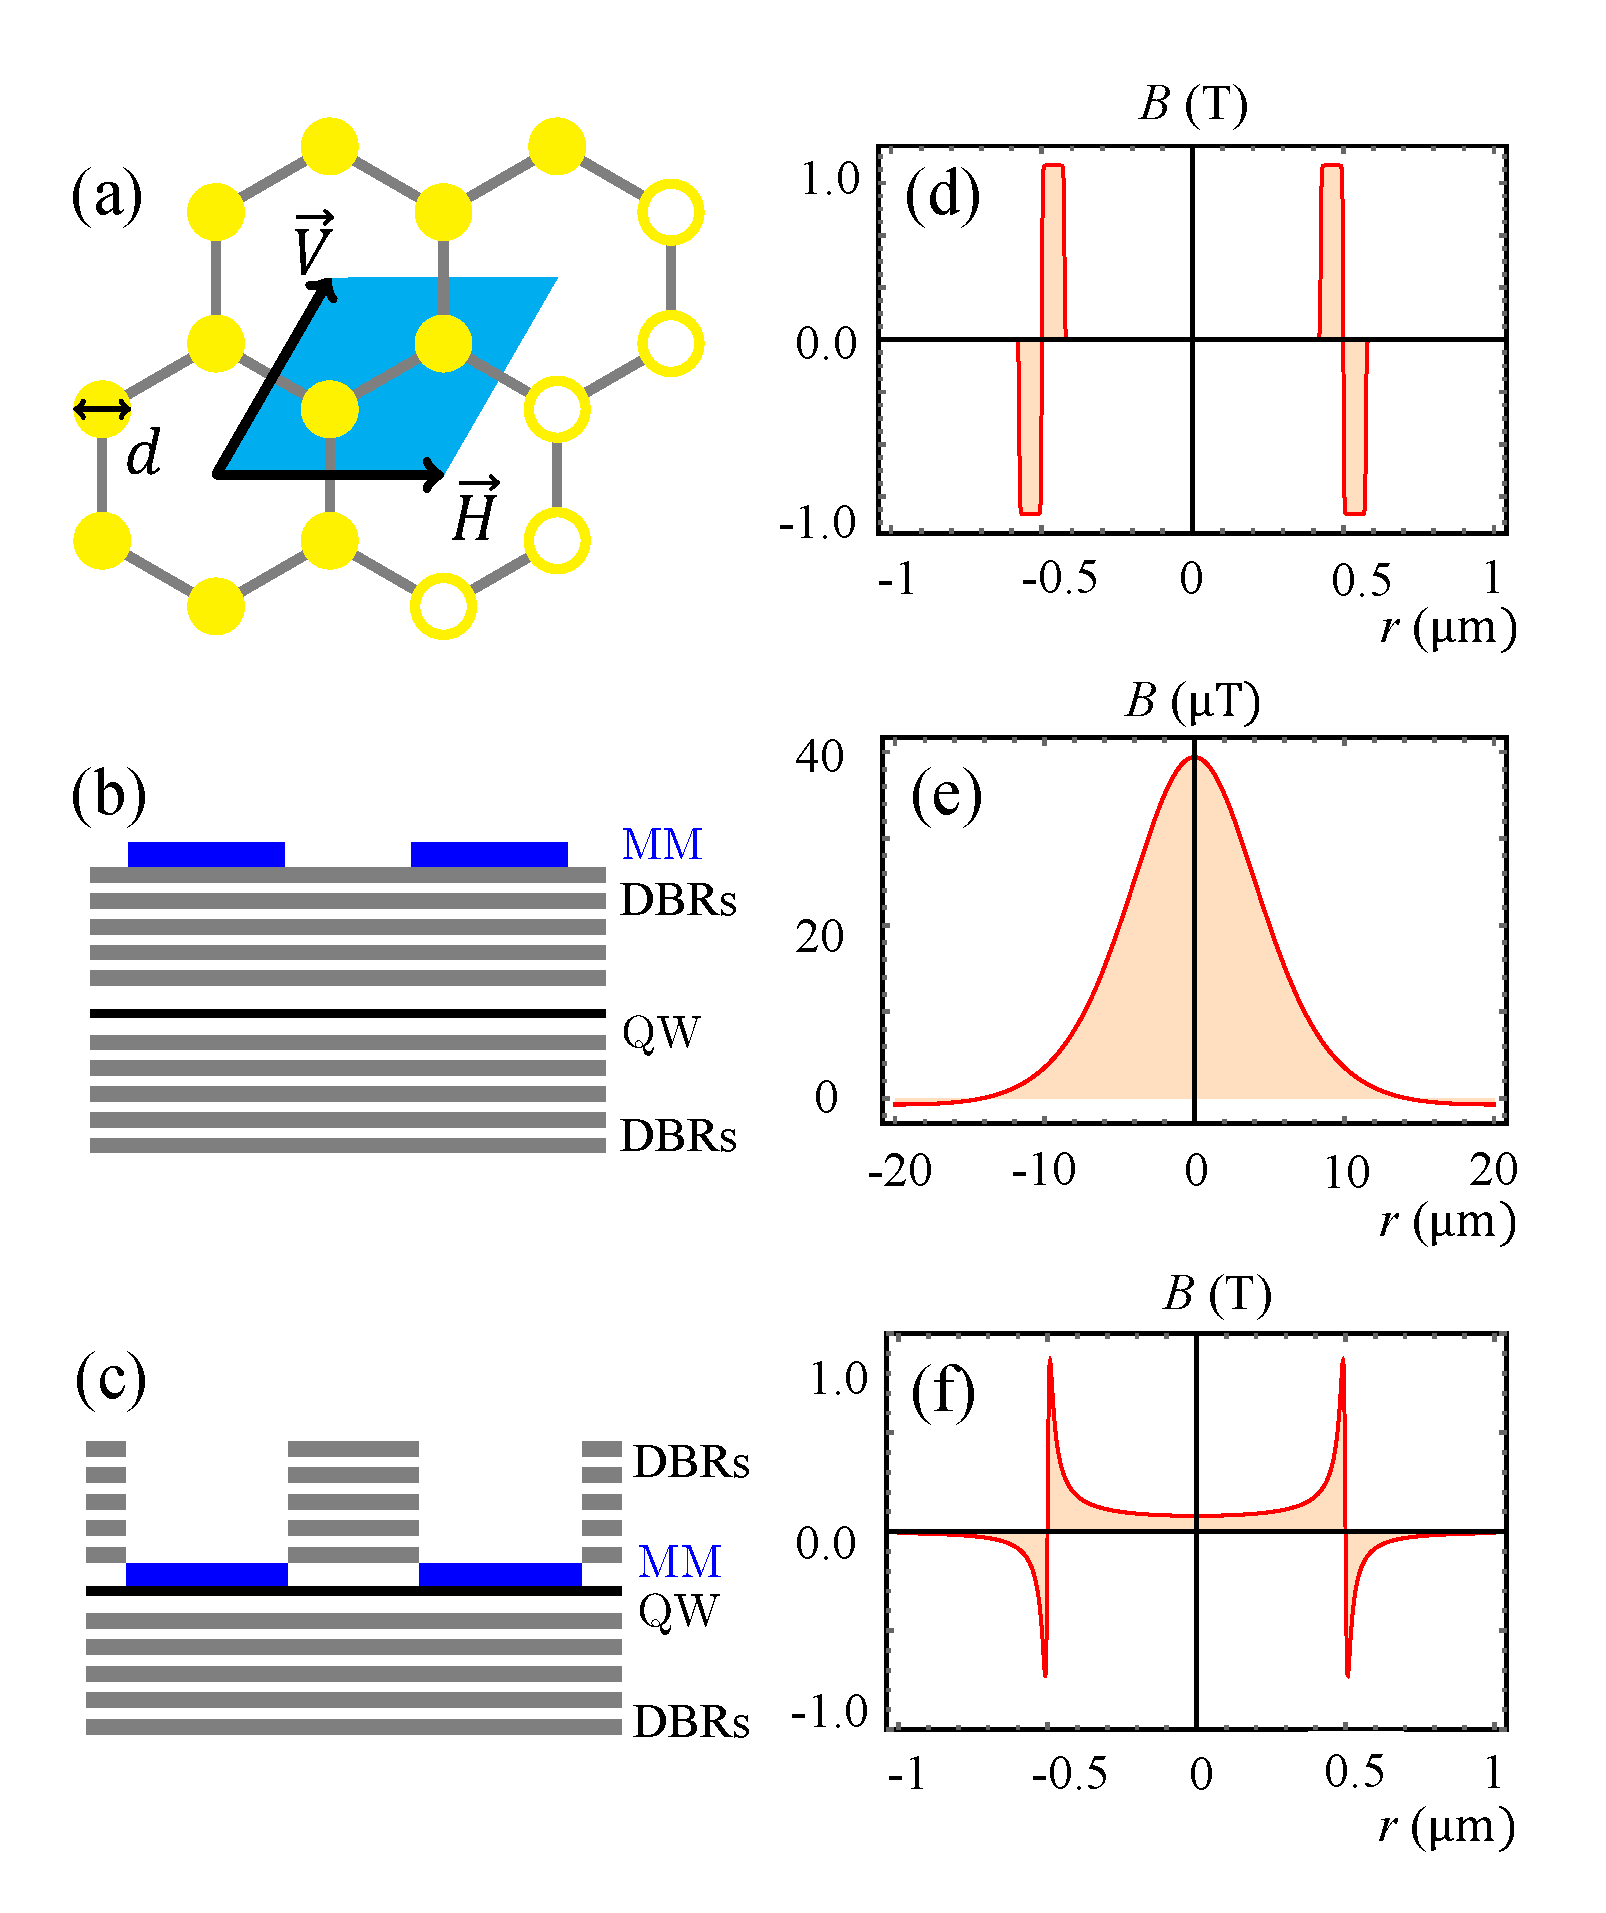
\includegraphics[width=0.55\textwidth]{Fig/Ch5/Fig1.pdf}
	\caption[TI system and magnetic field]{Left panels: System schematic: (a) A honeycomb lattice made of pillars of the etched cavity; yellow empty rings denote the region of the edge. The direction of the edge is along the $\vec{V}$ direction;
	(b) Setup using magnetic material (MM) placed on the top DBR;
	(c) Setup using MM placed at the top of the QW (close to the exciton layers).
	Right panels: Magnetic field profile in the case of a single MM disk with radius $R = 0.5$~$\mu$m  (d) Magnetic field used in numerical calculations, rectangle functions with width $dw$; (e) Magnetic field for case (b) and 10 $\mu$m away from the QW; (f) Magnetic field for case (c) and 8~nm away from the QW. The figure is taken from~\cite{Sun:2019ab}.}
\label{fig:Ch5_Fig1}
\end{figure}
%
%
%

The magnetic field from a single disc-shaped QD of radius $R$
%in the case without any screen effect due to superconductors
reads~\cite{Erdin:2002aa,Lyuksyutov:2005aa}
%
\begin{eqnarray}\label{eq:Ch5_EqDotMF}
B_z(r,z)=2\pi \mu_0 M R\int_0^\infty J_0(rq)J_1(Rq)\mathrm{e}^{-|z|q}q dq,
\end{eqnarray}
%
where $\mu_0 = 4\pi\times10^{-7} H/m$ is the vacuum permeability, $M=8\times 10^4Oe\cdot m$ is the 2D magnetization perpendicular to the disc-shaped QD, $J_i$ are the Bessel functions, $r$ is the distance from the center of the QD, $q$ is the in-plane momentum, and $z$ is the vertical distance from the MM to the QW.

The integral in Eq.~\eqref{eq:Ch5_EqDotMF} can be calculated semi-analytically, using special functions~\cite{A.-P.-Prudnikov:2003aa}, giving%
\begin{eqnarray}
B_z=\frac{\left[
f^2(R^2-r^2-z^2)E(f)
+(1-f^2)4rRK(f)
\right]}{4\mu_0^{-1}M^{-1} (Rr)^{3/2}(1-f^2)f^{-1}},~~ \label{eq:Ch5_Bfield}
\end{eqnarray}
%
where $f=\sqrt{\frac{4rR}{z^2+(r+R)^2}}$, and $K(f)$ and $E(f)$ are the elliptic integrals of the first and second kind, respectively.

Figure~\ref{fig:Ch5_Fig1}(e) shows the calculated profile of the $z$-projection of the magnetic field.
Since the distance between the layers of the excitons and the MM amounts to $z\sim$10 $\mu$m in this case (according to a typical size of a microcavity), the resulting effective magnetic field acting on the excitons is only of the order of $\mu$T, which is too small to create a useful topological bandgap. This is because $B_z$ in Eq.~\eqref{eq:Ch5_Bfield} decays exponentially with $z$.

To achieve a sufficient magnetic field, the separation between the MM and QW must be reduced.
For this, the scheme in Fig.~\ref{fig:Ch5_Fig1}(c) is considered, where the microcavity is etched to form a honeycomb lattice and an MM layer is deposited in the etched regions.
This allows the MM to be placed very close to the QWs, where the excitons reside, leading to interlayer separations of only $z \sim $1--20~nm and strong magnetic fields ($\sim 1$T).
The corresponding magnetic field profile [Fig.~\ref{fig:Ch5_Fig1}(f)] shows a rather different shape, as it is strongly localized at the micropillar/MM boundary, where it also changes sign.
Consequently, the magnetic field is said to be \emph{staggered} with zero net flux.
The profile in Fig.~\ref{fig:Ch5_Fig1}(f) is from a MM of radius $R=0.5\mu$m that produces a $\sim 1$~T magnetic field at a distance of 8~nm.

The process to fabricate this setup is as follows. First, grow the cavity with a multilayered structure. Second, etch micropillars to form the desired lattice potential. Third, deposit the MM onto the structure from the top. This way, part of the MM will be on the edges of the pillars.
However, as our calculations explicitly demonstrate, such remote sources of magnetic field will not substantially contribute and can therefore be neglected.
Lastly, by heating the sample above the Curie temperature and exposing it to a strong magnetic field, we can magnetize the sample and make it a permanent magnet.
%{\bf In this paragraph we should also state what MM we use to create the 1T field.}

%If, instead, we put the MM in between the pillars [see Fig.~1(c)], the distance amounts to only $z\sim$5-20~nm. In this case, the magnetic dots are replaced by a layer of MM with holes. And it can be grown very close to the quantum wells, where excitons reside. Thus a strong magnetic field is created [Fig.~1(f)].
%In what follows we will model it using an effective profile presented in Fig.~1(b).
%-----------------
%-----------------
%-----------------

\subsection{Transport of exciton-polaritons }
To determine the ability of this kind of staggered magnetic field configuration to create topological edge states, we numerically compute the band structure and Chern numbers of the polariton honeycomb lattice.
Due to computational limitations, we neglect the weak magnetic field inside and far away from the micropillars and approximate $B_z$ with a step function profile of width $dw$, as shown in Fig.~\ref{fig:Ch5_Fig1}(d).
%In order to calculate the band structure and the Chern numbers numerically, we use several simplifying approximation.
%In particular, we neglect the weak magnetic field in the middle and far away from the magnetic material between several neighboring pillars, thus give us several rectangle function with with $dw$ as shown in Fig.\ref{fig:Fig1}(b).
%
We describe the time evolution of the exciton-polaritons in the cavity by the Gross--Pitaevskii equation
%
\begin{eqnarray}
    \label{eq:Ch5_EOM}
    \mi\hbar \frac{\partial \psi_{\pm}}{\partial t} &=& -\frac{\hbar^2}{2m_{eff}}\nabla^2 \psi_{\pm} + V \psi_{\pm} + \Delta_{\pm}^{eff} \psi_{\pm} \nonumber \\
    &+& \beta^{eff} \left( \partial_x \mp \mi \partial_y \right)^2 \psi_\mp, \label{eq:Ch5_GPE}
\end{eqnarray}
%
where $\psi_\pm$ are the wave functions of polaritons with up- and down-polarization, $m_{eff}$ is the effective mass, the first term in the r.h.s. stands for the free particle propagation, $V$ is the potential of the honeycomb lattice with the lattice constant $3$~$\mu$m and site diameter $d = 0.75$~$\mu$m, and $\Delta^{eff}_\pm$ is the effective Zeeman splitting due to the presence of the MM with the shape presented in Fig.~\ref{fig:Ch5_Fig1}(d).
In the calculations, we first assume the lateral size of the MM to be the same as the well of the honeycomb lattice, and second, that the width of the rectangle functions is [Fig.~\ref{fig:Ch5_Fig1}(d)] $dw = 0.15$~$ \mu$m. Also, $\beta^{eff}$ is an effective TE-TM splitting.
We choose the Hopfield coefficients to be $\abs{X_H}^2 = 1 - \abs{C_H}^2 = 0.3$.
This gives us an effective polariton mass of $m_{eff} \approx m_C/\abs{C_H}^2$, with the effective mass of cavity photons as $m_C =3.23\cdot10^{-5}m_e$, where $m_e$ is free electron mass.
For polaritons, we have a similar (to excitons) definition of the effective Zeemann splitting and the TE-TM splitting: $\Delta_\pm^{eff} = \abs{X_H}^2 \Delta_\pm$ and $\beta^{eff} = \beta \abs{C_H}^2$.
In order to quantitatively estimate the magnetic field, we use the Zeeman splitting determined by the relation $\Delta_+-\Delta_- = g_x \mu_B |\mathbf{B}|$, where $g_x \mu_B\approx 180$~$\mu$eV$\cdot$T$^{-1}$ for excitons~\cite{Schneider:2013aa}.
As a result, for a Zeeman splitting term equaling $\Delta = \abs{\Delta_\pm}=1$~meV, the peak magnetic strength approximately equals to $5.5$~T, which means that the MM is $1$~nm away from the QW.


%----------------------------
%----------------------------
%----------------------------


\subsection{Phase diagram and edge modes}
First, we compute the bulk bands of Eq.~\eqref{eq:Ch5_GPE} by assuming a periodic structure and the Bloch wave Ansatz $\psi_{\pm} = u_{\pm}(\mathbf{k},\mathbf{r}) e^{\mi \mathbf{k}\cdot \mathbf{r} + \mi E t/\hbar}$.
Second, we find the bulk Bloch wave eigenstates and the Chern number~\cite{Fukui:2005aa} with
%
\begin{equation}
C =  \sum_{E_n < E_g} C_n = \frac{1}{2\pi \mi}\sum_{E_n < E_g} \oint_{\mathrm{BZ}}F_{\mu\nu}^n d^2k,
\label{eq:Ch5_Chern}
\end{equation}
%
where the Berry connection $A_n\left(k\right)$ ($n = 1,2$) in the $n$th band below the energy gap ($E_n<E_g$) and the associated field strength $F_{\mu\nu}\left(k\right)$ are defined as
%
\begin{eqnarray}
    A_\mu &=& \bra{n\left(k\right)}\partial_\mu\ket{n \left(k\right)},\nonumber \\
    F_{\mu\nu}\left(k\right) &=& \partial_\mu A_\nu\left(k\right) - \partial_\nu A_\mu\left(k\right),
\end{eqnarray}
%
where $\ket{n\left(k\right)} $ is the eigenvector of the $n$th Bloch band, and the inner product denotes integration over the unit cell.
Unit vector $\mu$ and $\nu$ denote the directions of the two reciprocal lattice vectors.
%{\bf Notation here can be cleaned up}

Solving Eq.~\eqref{eq:Ch5_Chern} for the system described in Eq.~\eqref{eq:Ch5_EOM}, we plot a Chern number diagram in Fig.~\ref{fig:Ch5_Fig2}(a), using the following parameters: $\Delta_\pm=\left[0.3\sim1.0\right]$~meV and a TE-TM splitting of $\beta = \left[ 0.1\sim0.3\right] $~meV$\mu$m$^{2}$.
As shown in the diagram, the system can possess different Chern numbers depending on the parameters. The phase transition between Chern numbers $C=2$ and $C=-1$ is due to a closing and opening of the gap at the $M$ point.
A similar behavior has been reported in~\cite{Bleu:2017aa} for the case of a homogeneous external magnetic field.

To confirm the existence of topological edge states, we also compute the energy spectrum of a semi-infinite structure (with 20 unit cells in the $\vec{H}$ direction and twisted boundary conditions in the $\vec{V}$ direction).
Typical spectra for the two topological phases are plotted in Fig.~\ref{fig:Ch5_Fig2}(b,c), which shows that the bulk bands and bandgaps host one and two edge states, respectively, in the gap between the second and third bands.
% The color of the edge mode stands for the polarization of the state: $I=\frac{\abs{\psi_+}^2-\abs{\psi_-}^2}{\abs{\psi_+}^2+\abs{\psi_-}^2}$. {\bf What does this polarization tell us?}
%
%
%
\begin{figure}[ht]
    \centering
    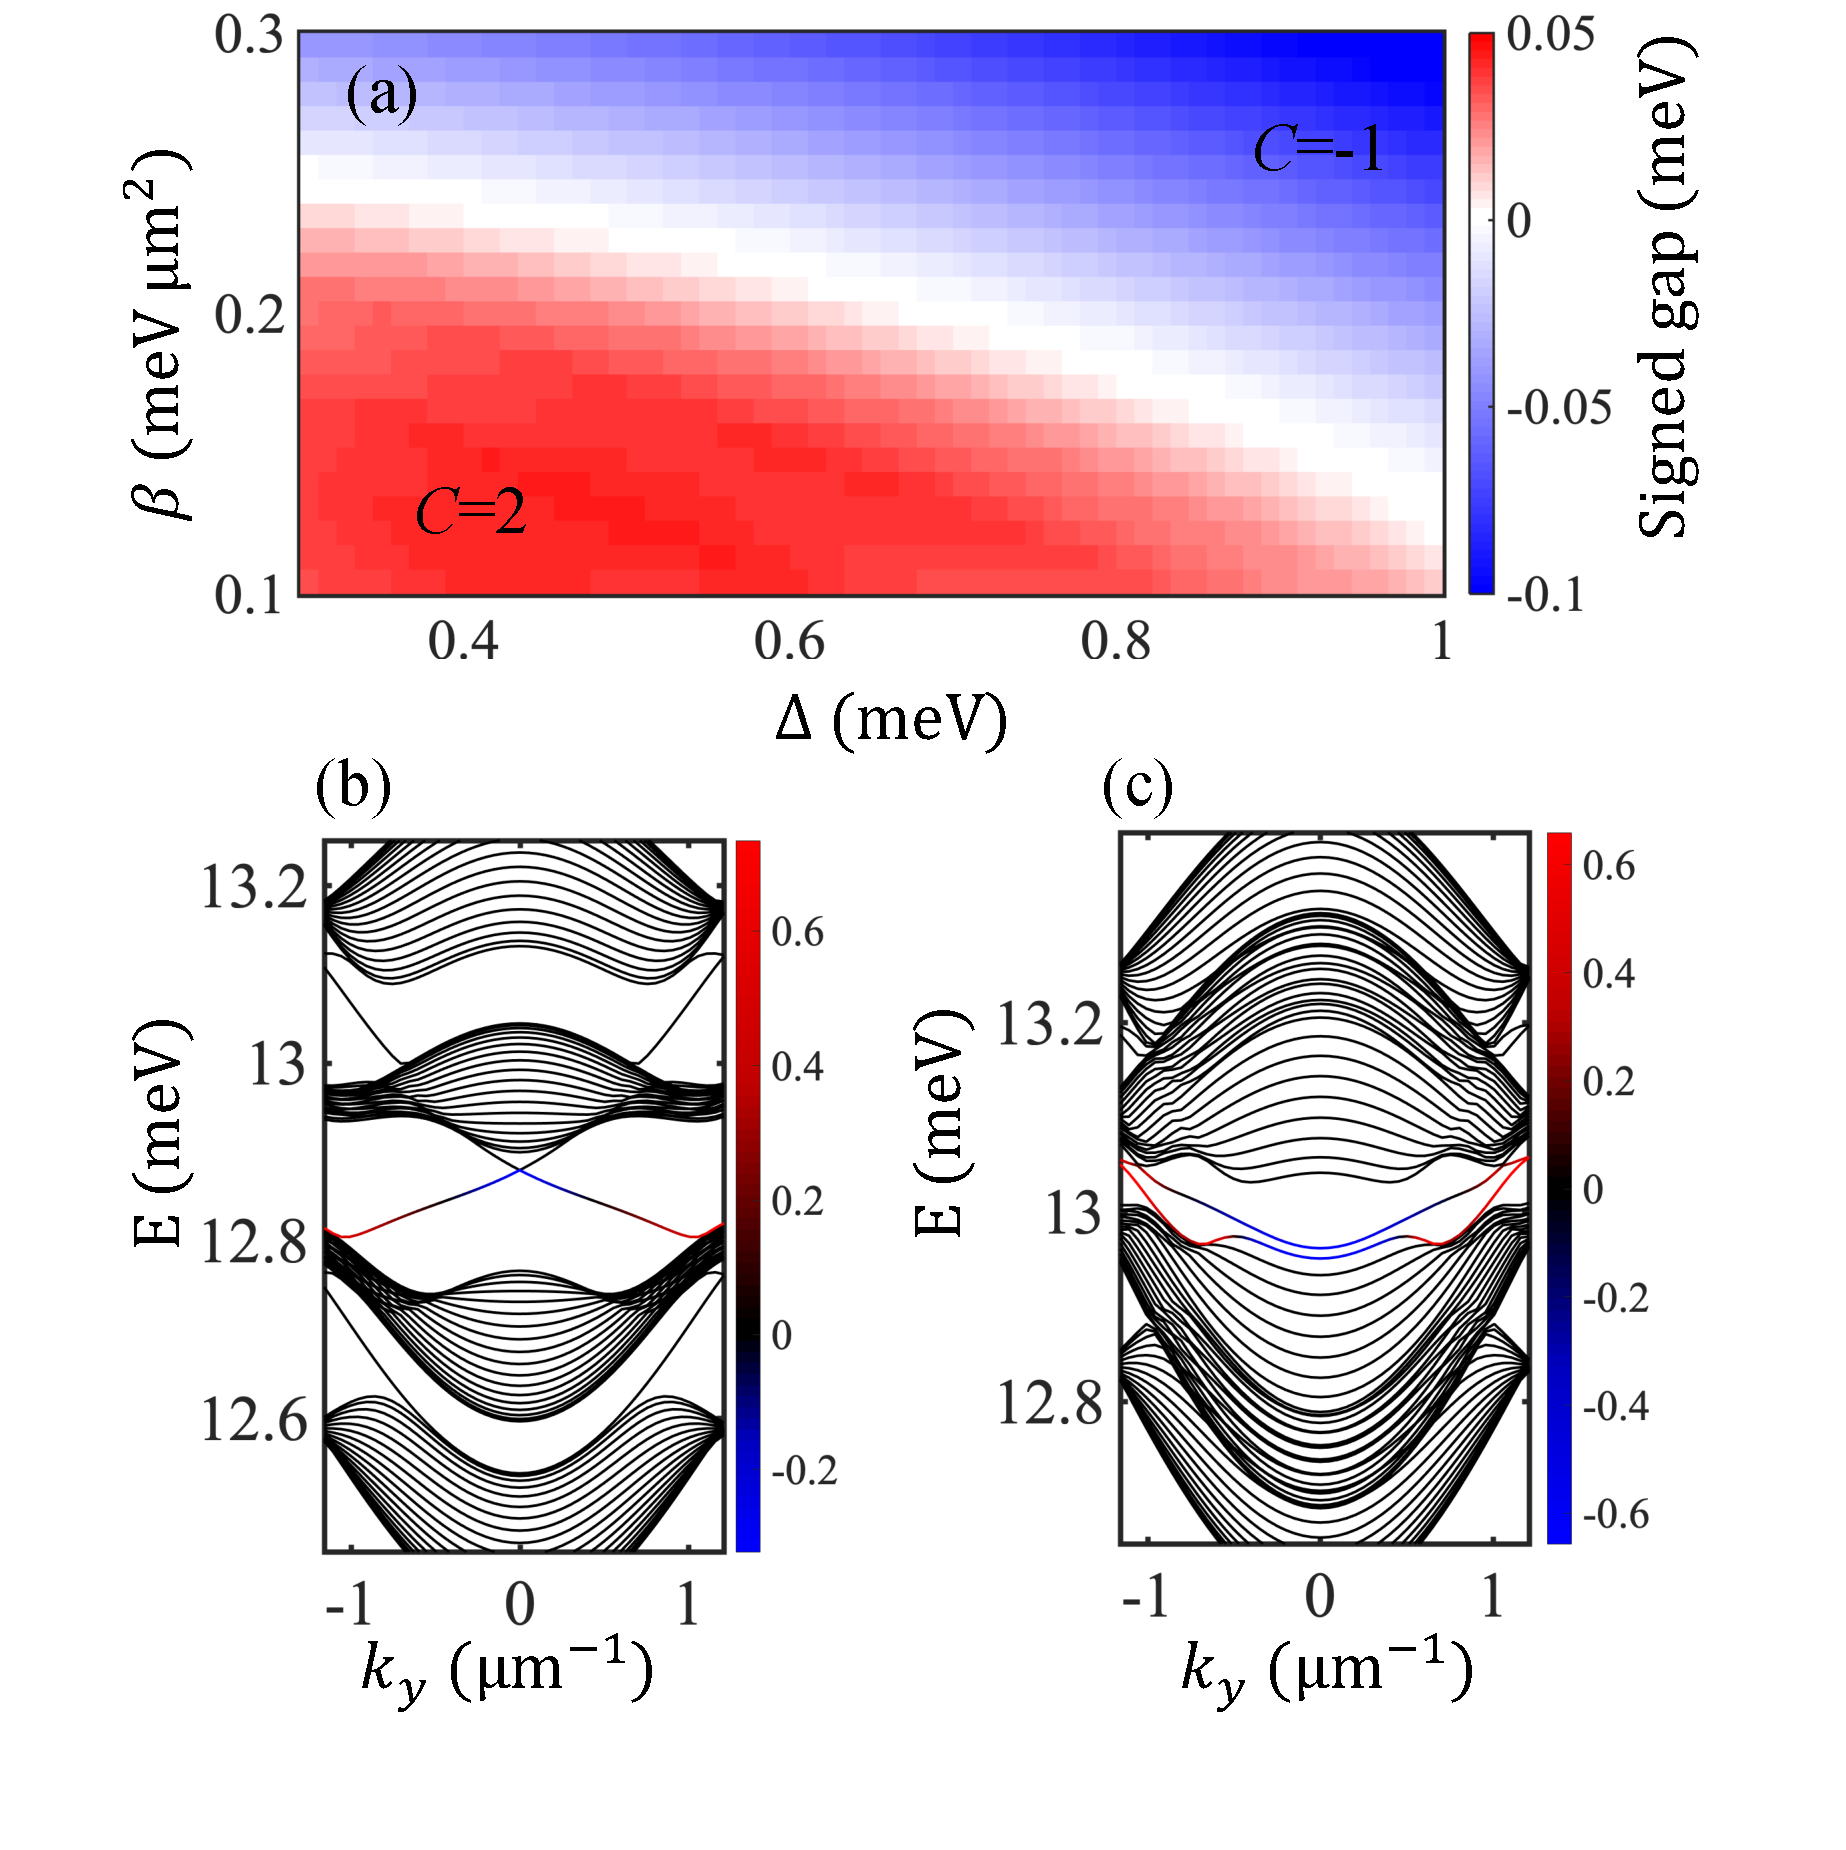
\includegraphics[width=0.55\textwidth]{Fig/Ch5/Fig2.pdf}%{fig2_new.pdf}
    \caption[Chern number phase diagram and edge states]{(a) Phase diagram for the Chern numbers with a TE-TM splitting of $0.1 \backsim 0.3$~meV$\mu$m$^2$ and a Zeeman splitting of $0.3 \backsim 1.0$~meV. The color bar indicates the size of the direct gap multiplied by the sign of the Chern number in units of meV. (b) and (c) Spectra of semi-infinite systems with Chern numbers $C = -1$ and $C = 2$, respectively. The color bar indicates the polarization imbalance $I = \frac{\abs{\psi_+}^2-\abs{\psi_-}^2}{\abs{\psi_+}^2+\abs{\psi_-}^2}$. For the $C=-1$ case, the edge mode is calculated at $\Delta=0.95$~meV and $\beta=0.27$~meV$\cdot\mu$m$^2$. For the $C=2$ case, the edge mode is calculated at $\Delta=0.46$~meV and $\beta=0.13$~meV$\mu$m$^2$. The figure is taken from~\cite{Sun:2019ab}.}
    \label{fig:Ch5_Fig2}
\end{figure}
%
%
%
%--------------------
%--------------------
%--------------------

\subsection{Comparison with the homogeneous case}
One key difference between systems with MM and with an external magnetic field is the magnitude of the magnetic flux.
In the MM case, on account of the strong localization of the magnetic field, the total net flux within one unit cell is almost zero.
%Therefore, for comparison we define the absolute value of the flux on the plane by an integral over a single unit cell:
To compare the MM and the external magnetic field cases, we define the absolute value of the flux on the plane by the integral over a single unit cell region as
%
\begin{equation}
    \Phi = \frac{\oint_S \abs{{\Delta_{\pm}}}ds}{S},
\end{equation}
%
where $S$ is the area of the unit cell.
Since the Zeeman splitting is proportional to the magnetic field, we can compare the bandgaps between the 2nd and 3rd levels as functions of the absolute flux, $\Phi$, in the two cases.
We assume that the direction of the magnetic field is the same as the direction of the outer edge of the MM.
Figure~\ref{fig:Ch5_gap}(a) shows that, given the same value of the absolute magnetic flux, the gap closes and reopens in a similar manner.

Alternatively, we can compare the magnitude of the gap as a function of the peak value of the magnetic field, i.e., the peak intensity of the Zeeman splitting.
Figure~\ref{fig:Ch5_gap}(b) demonstrates the sizes of the gaps in the MM and homogeneous cases as functions of the peak value of the Zeeman splitting.
We also label the Chern numbers in both cases before and after the gap is closed.
In the homogeneous case, the gap closes much earlier than in the MM case.
%
%
%
\begin{figure}[ht]
    \centering
    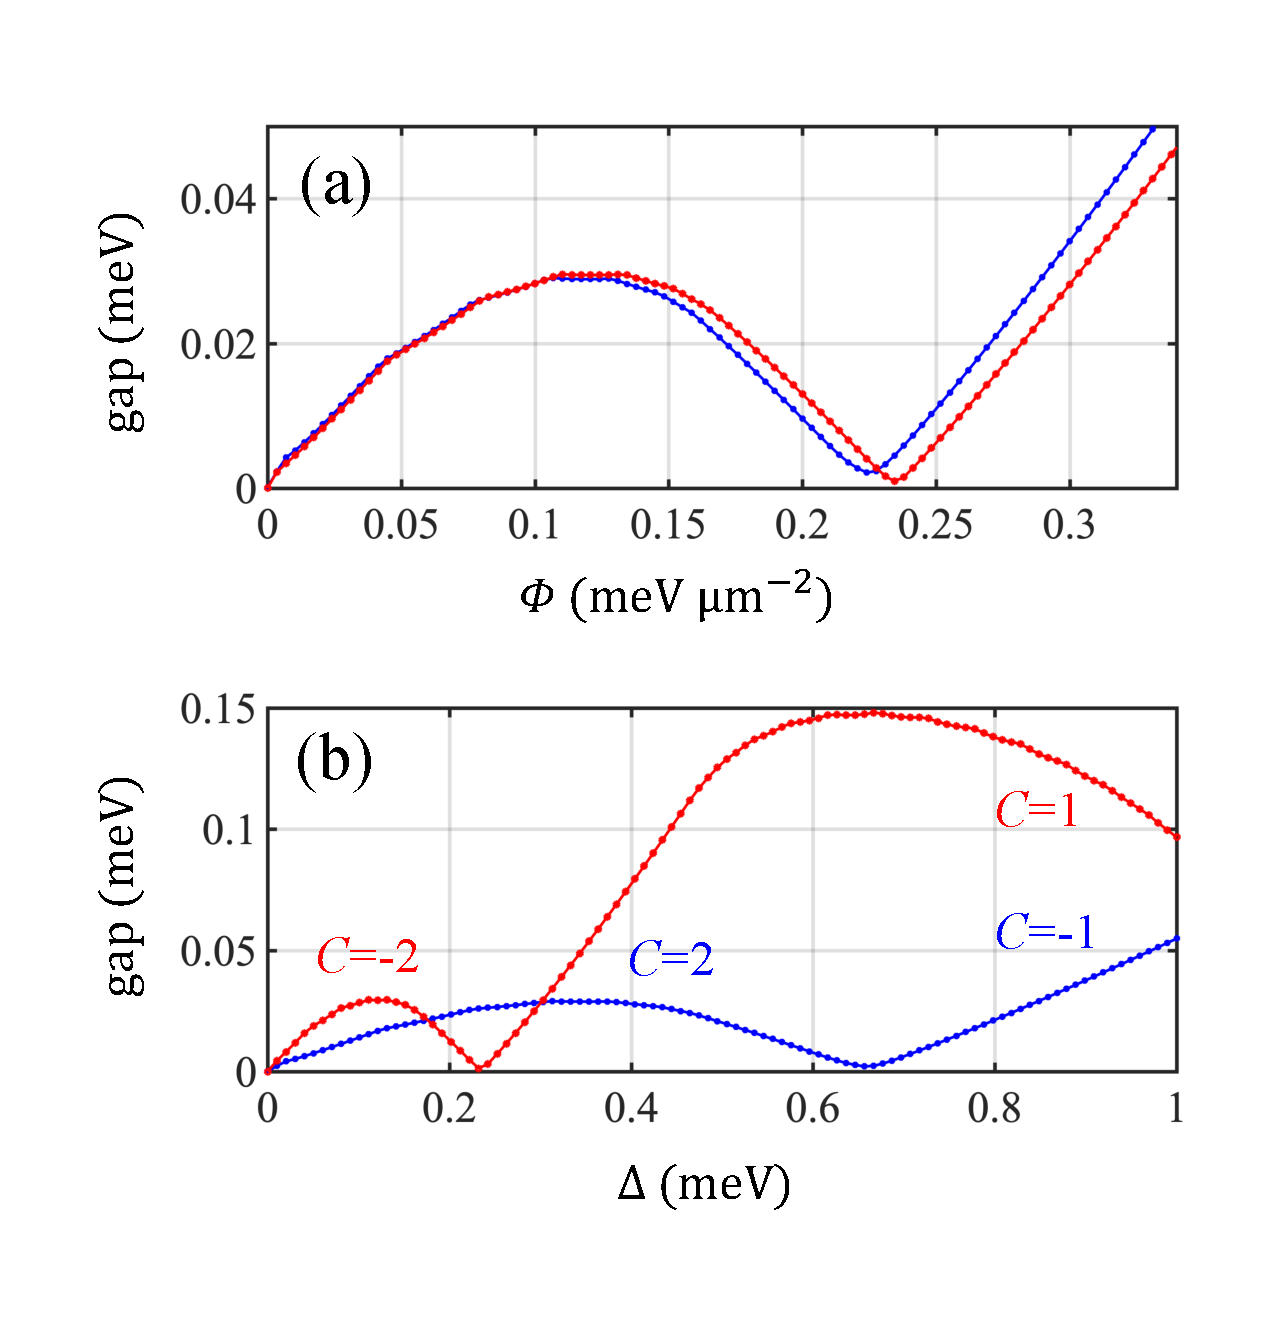
\includegraphics[width=0.45\textwidth]{Fig/Ch5/Fig3.pdf}
    \caption[Bandgap between MM and external magnetic field]{(a) Bandgap as a function of the absolute flux. (b) Bandgap as a function of the peak value of the Zeeman splitting. Blue and red lines show the MM and homogeneous magnetic field cases, respectively. The TE-TM splitting is fixed to $\beta = 0.2$~meV$\cdot\mu$m$^2$. The figure is taken from~\cite{Sun:2019ab}.}
    \label{fig:Ch5_gap}
\end{figure}
%
%
%


%--------------------
%--------------------
%--------------------

\subsection{Cavity with a MM exposed to an external magnetic field}
With MM embedded in a cavity, a homogeneous magnetic field can still be applied to the sample. In this case, the resulting field represents a superposition of two magnetic field profiles (Fig.~\ref{fig:Ch5_fig4}).

The first case to consider is one in which the external magnetic field $\mathbf{B}_{ex}$ is parallel to the outside edge of the MM, $\mathbf{B}_{MM}$, as shown in the inset of Fig.~\ref{fig:Ch5_fig4}(a).
Here, we see an additional phase transition in red and green curves.
Specifically, we can classify two distinct regimes.
The first one is when the MM is weak ($\Delta < 0.2$~meV). With an increasing homogeneous magnetic field ($\Delta_{ex}$, from green to red curve), the system undergoes a phase transition from Chern number $C=-2$ to $C=1$.
The second one is when the MM is moderately strong ($0.3$~meV$<\Delta<0.8$~meV), in which the Chern number changes from $C=2$ to $C=-2$ as $\Delta_{ex}$ increases.

The second case is the antiparallel case as shown in Figure~\ref{fig:Ch5_fig4}(b).
Red and blue curves show that the gap size in the $C=-1$ case can be efficiently enlarged.
Gap sizes are vital in topological polaritonic systems, since the finite lifetime of the exciton-polaritons can broaden the bandwidth of the spectrum and diminish and destroy nontrivial topological properties.
We conclude that the combination of the two magnetic fields reduces the required strength of the external magnetic field to generate a topological insulator state with a given bandgap.
%
%
%
\begin{figure}[ht]
\centering
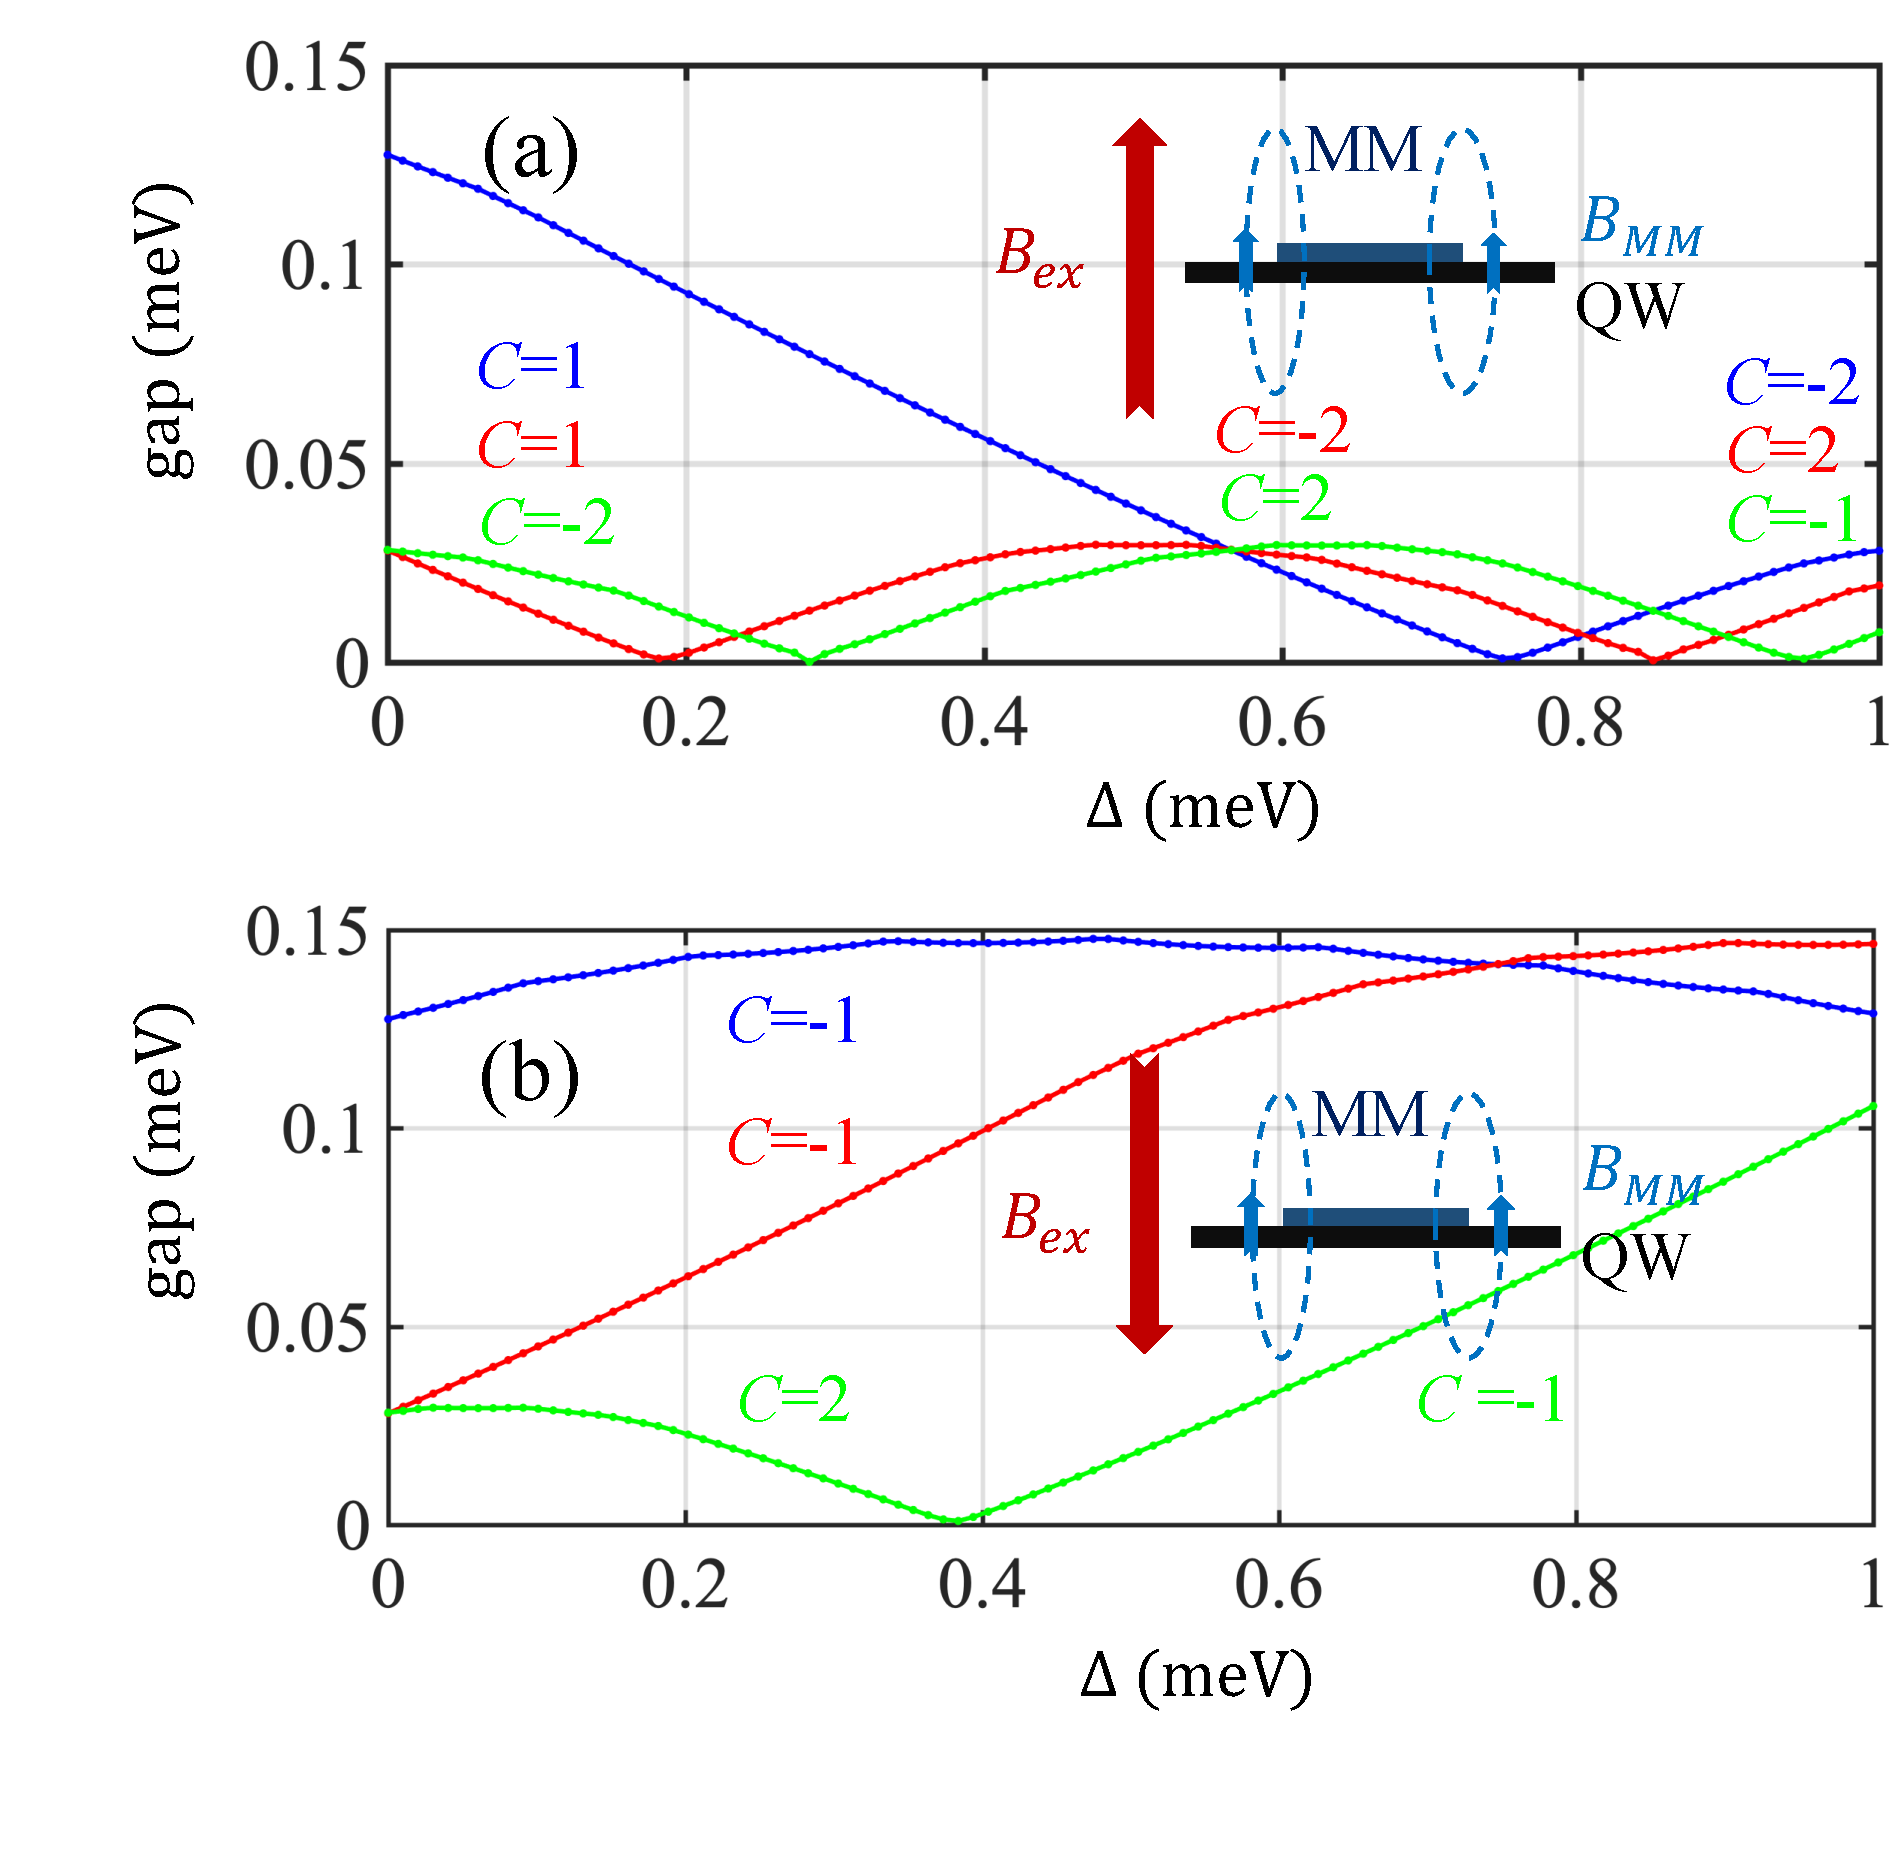
\includegraphics[width=0.45\textwidth]{Fig/Ch5/Fig4.pdf}
\caption[Bandgap of MM under external magnetic field]{The mutual effect of MM and an external magnetic field with (a) parallel and (b) antiparallel magnetic field directions, as drawn in the insets.
The x-axis is the intensity of the local magnetic field of MM.
Different colors reflect different magnitudes of external magnetic field,
$B_{ex}\approx 2.8$, $1.7$, and $0.5$~T, corresponding to the Zeeman splittings $\Delta_{ex}=0.5$ (blue), $0.3$ (red), and $0.1$~meV (green).
The Chern numbers are labeled before and after each gap.
The TE-TM splitting is fixed at $\beta = 0.2$~meV$\cdot\mu$m$^2$. The figure is taken from~\cite{Sun:2019ab}.}
    \label{fig:Ch5_fig4}
\end{figure}
%
%
%


%---------------------------
%---------------------------
%---------------------------

%\pagebreak

\subsection{Discussion}
This Chapter showed that a local magnetic field from the presence of a magnetic material can be sufficiently strong to open a gap at the Dirac point and allow for the observation of nontrivial topological states in an exciton-polariton system loaded in a honeycomb lattice.
With intensity changes of the embedded magnetic field or TE-TM splitting, the system undergoes a phase transition between two nontrivial states with the Chern numbers $\pm2$ and $\mp1$.

The key advantage of this setup is the size of the system, which can be much smaller than those requiring a homogeneous external magnetic field.
This can be highly beneficial for future experiments and device applications.
Furthermore, we have studied the Chern numbers and gap sizes as functions of the magnetic flux strength and the peak value of the magnetic field, with results showing that designs utilizing MM and a regular homogeneous field both demonstrate similar behavior.

Next, the joint effect of an internal MM field with an external magnetic field was explored.
Depending on the relative direction of the two fields, one can switch between different Chern numbers.
This switching can be performed ``on the fly", since it depends only on a small change of the external magnetic field, thereby enabling control over the number and/or the direction of the topological edge states.
By reversing the direction of the external magnetic field, one can also keep the Chern number the same but enlarge the size of the gap significantly, thus increasing the speed of the edge state.
This allows us to propagate polaritons over longer distances before they decay due to their finite lifetime.
